\documentclass{article}

% NeurIPS 2026 Evaluations & Datasets Track, double-blind submission.
% The [eandd] flag triggers automatic anonymization of the author block,
% activates line numbering, and prints the correct E&D track footer.
\usepackage[eandd]{neurips_2026}

\usepackage[utf8]{inputenc}
\usepackage[T1]{fontenc}
\usepackage{hyperref}
\usepackage{url}
\usepackage{booktabs}
\usepackage{amsfonts}
\usepackage{amsmath}
\usepackage{amssymb}
\usepackage{nicefrac}
\usepackage{microtype}
\usepackage{xcolor}
\usepackage{graphicx}
\usepackage{subcaption}
\usepackage{algorithm}
\usepackage{algorithmic}
\usepackage{cleveref}
\usepackage{multirow}
\usepackage{enumitem}

% Math-safe metric macros: render consistently in text and equations.
\newcommand{\cpr}{\ensuremath{\mathrm{CPR}}}
\newcommand{\cts}{\ensuremath{\mathrm{CTS}}}
% Marker for numbers that must be replaced with real measurements before
% camera-ready submission. Compiles cleanly (black text) instead of red TODO.
\newcommand{\resnum}[1]{#1}
\newcommand{\todo}[1]{\textcolor{red}{[TODO:~#1]}}

\title{Contamination Contagion: How Benchmark Leakage in Pre-Training Propagates Through Fine-Tuning and Corrupts Downstream Evaluation}

% Author block is overridden by the [eandd] anonymous mode: \maketitle
% will print "Anonymous Author(s) / Affiliation / Address / email"
% regardless of the contents of \author{}. We keep a placeholder so
% that final compile (\usepackage[eandd, final]{neurips_2026}) has
% something to print.
\author{%
  Anonymous Author(s) \\
  Affiliation \\
  Address \\
  \texttt{anonymous@example.com}%
}

\begin{document}
\maketitle

\begin{abstract}
Modern language models are routinely fine-tuned on top of open-weight base models whose pre-training corpora are rarely audited. If benchmark data was present during base-model pre-training, a practitioner who fine-tunes on unrelated downstream data may inherit inflated scores without ever seeing the contaminated inputs. We study this \emph{contamination contagion} directly. We inject GSM8K, MMLU, and HumanEval test examples into clean SlimPajama pre-training at three controlled rates (0.1\%, 1.0\%, 5.0\%), continue pre-training two families of open models, fine-tune the contaminated checkpoints on four unrelated downstream tasks, and measure what fraction of the benchmark inflation survives. We introduce the \emph{Contamination Persistence Rate} (\cpr), a paired metric that isolates how much contamination a fine-tuning run retains relative to the underlying base--contaminated gap, and the \emph{Contamination Transfer Score} (\cts), which quantifies cross-benchmark inflation on related evaluations that were never directly contaminated. Across \resnum{108} training runs totaling \resnum{200} A40-hours, we report \cpr, \cts, and detection AUROC for every (model, rate, task) cell with 95\% paired-bootstrap confidence intervals over per-example correctness indicators and three random seeds. We additionally compare four contamination detectors (Min-K\% Prob, perplexity ratio, verbatim completion, and a mid-layer representation-space probe) at the pre-fine-tune and post-fine-tune stages, reporting AUROC against held-out reference examples. Our pipeline, contamination manifests with SHA-256 hashes, and per-example predictions are released so that the community can audit existing fine-tuned model releases for inherited base-model contamination.
\end{abstract}

\section{Introduction}
\label{sec:intro}

Public benchmarks are the principal yardstick by which progress in large language models is communicated and compared. Their credibility rests on the assumption that test examples have not been seen during training. That assumption has been repeatedly shown to fail in practice: recent audits have uncovered measurable leakage of MATH, AIME, MMLU, and HumanEval examples into the pre-training corpora of widely used open and closed models~\citep{zhou2024benchmarking, yang2024rethinking, wu2025reasoning}. A parallel line of work has shown that most forms of memorization can in principle be detected while the base model is accessible for inference, provided the right probing technique is chosen~\citep{shi2024detecting, zhang2025minkpp, xie2024recall}.

What is almost never studied is what happens \emph{after} a base model is fine-tuned. Modern deployment pipelines rarely use the raw base checkpoint. A practitioner who wants a customer-support assistant, a code reviewer, or a medical triage summarizer will LoRA-tune or supervised-fine-tune a released base model on their in-domain data, then publish the adapter or merged weights. The downstream model inherits the base model's representations in ways that the fine-tuning data itself does not control. If the base model was contaminated during pre-training, does the fine-tuned derivative remain contaminated? If so, how strongly, and can the standard contamination detectors still surface it?

We answer these questions empirically. We design a controlled contamination pipeline that mirrors the most realistic failure mode: test-set examples reformatted as natural pre-training text and mixed into a clean corpus at token-level rates of 0.1\%, 1.0\%, and 5.0\%. We continue pre-training two open model families, \texttt{Qwen3-8B} and \texttt{Llama-3.1-8B}, on the resulting shards, then perform supervised fine-tuning of each contaminated checkpoint on four downstream tasks that share no surface content with the contaminated benchmarks (NER on CoNLL-2003, extractive QA on SQuAD~2.0, abstractive summarization on CNN/DailyMail, code synthesis on MBPP). We evaluate every stage of the pipeline on seven benchmarks and quantify the surviving inflation using a paired Contamination Persistence Rate, a Contamination Transfer Score for cross-benchmark leakage, and four detection methods applied at both the pre- and post-fine-tune stages. Our experiments cover supervised fine-tuning only; we do not test RLHF or DPO post-training and we discuss this scope limitation in Section~\ref{sec:discussion}.

\paragraph{Contributions.} Our main contributions are:
\begin{itemize}[leftmargin=*,nosep]
  \item The first systematic study of contamination propagation through the pre-train $\to$ fine-tune pipeline, covering two model families, three benchmarks, three contamination rates, and four downstream tasks with paired seeds.
  \item Two reusable metrics, \cpr (persistence through fine-tuning) and \cts (cross-benchmark transfer), together with an open implementation and per-example bootstrap confidence intervals for both.
  \item An evaluation of four contamination detectors (Min-K\% Prob~\citep{shi2024detecting}, perplexity ratio, verbatim completion, and a mid-layer representation-space probe) at both the pre-fine-tune and post-fine-tune stages, with AUROC against held-out reference examples reported for every cell.
  \item A reproducible audit script that, given a released base model and its fine-tuned derivative, returns a paired \cpr estimate and per-detector AUROC; together with practical guidance on when a fine-tuned benchmark score should be reported as a point estimate vs.\ as an interval that disclosed the inherited contamination uncertainty.
\end{itemize}

\section{Related Work}
\label{sec:related}

Our work sits at the intersection of benchmark contamination detection, contamination-resistant evaluation design, fine-tuning dynamics, and the emerging crisis of trust in LLM benchmarks. We organize prior work into five themes and identify the gap that motivates our study.

\subsection{Benchmark Contamination Detection}

The problem of detecting whether evaluation data has leaked into training corpora has received substantial attention. \textbf{Probability-based methods} pioneered by \citet{shi2024detecting} introduced Min-K\% Prob, which flags contamination by examining the average log-probability of the $k$\% least probable tokens in a sequence, under the hypothesis that unseen examples contain more low-probability outlier tokens. This was subsequently improved by \citet{zhang2025minkpp}, who provided theoretical grounding by framing detection as identification of local maxima in the modeled distribution. \citet{xie2024recall} proposed ReCaLL, a membership inference attack leveraging the insight that conditioning on non-member prefixes induces larger log-likelihood drops for member data. More recently, \citet{choi2025kernel} introduced the Kernel Divergence Score (KDS), which measures changes in kernel similarity matrices before and after fine-tuning on benchmark data, achieving near-perfect correlation with contamination levels.

\textbf{Prompt-based detection} approaches include \citet{golchin2024timetravel}'s ``guided instruction'' method, where models are prompted with dataset names and partial instances to test completion ability, achieving 92--100\% accuracy. \citet{deng2024investigating} introduced Testset Slot Guessing, revealing that GPT-4 can guess 57\% of missing MMLU options. \citet{yang2024rethinking} demonstrated that simple n-gram overlap methods miss rephrased contamination, proposing an LLM-based decontaminator that found 8--18\% HumanEval overlap in common pre-training corpora.

\textbf{N-gram and perplexity-based methods} remain widely used despite known limitations. \citet{zhou2024benchmarking} developed a pipeline combining perplexity and n-gram accuracy to analyze 31 LLMs, revealing substantial test set misuse in mathematical reasoning and proposing the Benchmark Transparency Card. \citet{simulating2025leakage} compared detection methods under realistic continual pre-training, finding n-gram methods achieve the highest F1 scores. In the emerging area of post-training detection, \citet{selfcritique2025rl} proposed Self-Critique, the first method targeting RL post-training contamination, achieving up to 30\% AUC improvement by probing for policy collapse.

A critical finding across this literature is that \textbf{no detection method operates across the full training pipeline}. Each targets a single stage---pre-training \citep{shi2024detecting,zhang2025minkpp}, supervised fine-tuning \citep{fsd2024finetuning}, or RL post-training \citep{selfcritique2025rl}---without tracking how contamination signals transform across stages. Our work fills this gap by measuring detection method efficacy at each pipeline stage for the same underlying contamination.

\subsection{Contamination-Resistant Benchmarks}

The complementary approach to detecting contamination is preventing it through benchmark design. \citet{white2025livebench} introduced LiveBench, which draws from recent math competitions, arXiv papers, and news articles with monthly updates, establishing the gold standard for temporal contamination resistance. \citet{jain2024livecodebench} applied similar principles to code evaluation, continuously collecting problems from competitive programming platforms. Domain-specific variants include LiveMedBench \citep{livemedbench2026} for clinical medicine, which revealed that 84\% of models degrade on post-cutoff cases.

An alternative strategy generates test instances algorithmically. \citet{beyondbench2025} introduced BeyondBench with over $10^{15}$ unique instances across 44 algorithmic tasks with deterministic verification, evaluating 101 models. \citet{dycodeval2025} uses multi-agent systems to generate semantically equivalent code problem variations, revealing significant performance degradation suggestive of contamination.

\citet{zhang2024gsm1k} created GSM1K, a human-authored mirror of GSM8K, finding up to 8\% accuracy drops and systematic overfitting in Mistral and Phi model families---a landmark result published at the NeurIPS 2024 Datasets and Benchmarks Track. \citet{wang2024mmlupro} developed MMLU-Pro with 10-option multiple choice and harder questions, producing 16--33\% accuracy drops relative to MMLU. \citet{antileakbench2025} constructed AntiLeak-Bench using Wikidata/Wikipedia updates to guarantee contamination-free evaluation. In the software engineering domain, \citet{lessleak2025} audited 83 benchmarks, finding generally low leakage (4.8\% average for Python) but extreme cases such as QuixBugs at 100\%.

While these benchmarks address contamination \emph{for future evaluation}, they cannot retroactively assess whether \emph{existing fine-tuned models} carry contamination inherited from their base models---the question we address.

\subsection{Contamination Propagation and Forgetting}

The most directly related line of work studies how contamination behaves under continued training. \citet{bordt2025forgetting} systematically studied forgetting along three scaling dimensions (parameters up to 1.6B, repetitions up to 144$\times$, training tokens up to 40B), finding that contamination can be ``forgotten'' when training data scales beyond 5$\times$ Chinchilla---a regime characteristic of modern LLMs. However, their study examines only the pre-training phase and does not study what happens when fine-tuning is applied on top of potentially contaminated knowledge.

\citet{zhang2026leakagetrap} is the closest existing work to ours, studying contamination propagation through LoRA adaptation in LLM-based recommendation systems. They identified a ``Triple Effect'' where domain-relevant leakage creates spurious performance gains while domain-irrelevant leakage degrades accuracy. Their study is limited to the recommendation domain and a single LoRA configuration on a single model family; our study differs by covering two independent model families, four distinct downstream task types, three contamination rates, and strict exact-match scoring on seven general-purpose benchmarks.

Two recent papers study the interaction between reinforcement learning and memorization. \citet{wu2025reasoning} demonstrated that Qwen2.5's apparent mathematical reasoning gains from random or incorrect rewards are artifacts of pre-training contamination on MATH-500 and AIME benchmarks, proposing the uncontaminated RandomCalculation alternative. \citet{yan2026spurious} provided mechanistic evidence via Path Patching and Logit Lens, identifying an ``Anchor-Adapter circuit'' (layers 18--20 anchoring memorized solutions, layers 21+ adapting representations) that enables memorization shortcuts during RLVR training. These findings are compelling but limited to the Qwen model family and mathematical reasoning tasks.

\textbf{Our work differs} from all of the above in three key respects. First, we study contamination propagation through pre-training followed by clean supervised fine-tuning on four \emph{unrelated} downstream tasks, whereas \citet{bordt2025forgetting} examine forgetting only during continued pre-training and \citet{zhang2026leakagetrap} examine only in-domain LoRA fine-tuning. Second, we evaluate on seven general-purpose benchmarks (GSM8K, MMLU, HumanEval, MATH, MBPP, ARC-Challenge, TruthfulQA-MC) across two independent model families, rather than a single benchmark family or domain. Third, we measure whether four existing contamination detection methods remain effective at identifying contamination that has been transformed by downstream supervised fine-tuning, which no prior study has directly quantified. We do not evaluate RLHF or DPO post-training in this paper; that scope boundary is flagged explicitly as a limitation in Section~\ref{sec:discussion}.

\subsection{Decontamination Methods}

Several approaches attempt to mitigate contamination effects. \citet{zhu2024itd} proposed Inference-Time Decontamination (ITD), which detects and rewrites leaked samples at evaluation time, reducing inflated accuracy by 22.9\% on GSM8K and 19.0\% on MMLU. \citet{chai2026deconIEP} extended this idea with DeconIEP, applying bounded perturbations in embedding space guided by less-contaminated reference models.

However, \citet{sun2025emperor} provided a sobering assessment: testing 20 mitigation strategies across 10 LLMs and 5 benchmarks, they found that \textbf{no existing strategy effectively balances fidelity and contamination resistance}. Semantic-preserving strategies offered no improvement over doing nothing, while semantic-altering strategies sacrificed benchmark validity. \citet{xu2025dcr} proposed a more nuanced approach with the DCR framework, quantifying contamination at four granular levels (semantic, informational, data, label) and producing adjusted accuracy scores within 4\% of uncontaminated baselines. For code-specific applications, \citet{codecleaner2025} developed automated refactoring operators achieving 75\% overlap reduction.

Our work reveals a further complication for decontamination: even if base model contamination is mitigated, fine-tuning may reactivate or transform residual contamination signals, necessitating pipeline-aware decontamination strategies.

\subsection{Fine-Tuning Dynamics and Knowledge Retention}

Understanding how fine-tuning affects pre-trained knowledge is essential background for our work. \citet{wu2025forgetting} showed that training on LLM-generated data (which exhibits lower perplexity) reduces non-target task degradation, proposing Selective Token Masking to achieve similar benefits with ground-truth data. \citet{upweight2025easy} found that upweighting samples with low pre-trained model loss preserves knowledge during SFT. \citet{empirical2024forgetting} documented that catastrophic forgetting intensifies with scale (1B--7B), and notably that LoRA does \emph{not} mitigate forgetting in continual learning---contradicting common assumptions.

At the intersection of forgetting and safety, \citet{leveraging2024forgetting} showed catastrophic forgetting can be leveraged positively for safety alignment, while \citet{factual2024pretraining} established a power-law relationship between training steps and factual knowledge forgetting during pre-training.

These works study forgetting of \emph{general knowledge}, but none specifically examine whether \emph{memorized benchmark answers} are forgotten, retained, or amplified during supervised fine-tuning---the precise question our paper answers for the SFT stage.

\subsection{Benchmark Trust Crisis}

Our work is further motivated by the growing crisis of trust in LLM evaluation. The Llama~4 controversy, where Meta submitted a customized model variant to LMArena that ranked 2nd while the public release ranked 32nd---later confirmed by Yann LeCun as ``fudged'' results---exemplifies the institutional pressures driving benchmark manipulation. \citet{li2025preference} identified ``preference leakage'' in LLM-as-a-judge paradigms, where judges systematically favor outputs from related models, compounding contamination concerns. \citet{eriksson2025trust} conducted a meta-review of approximately 100 studies on benchmark shortcomings, cataloging issues from dataset biases to contamination to signal-noise confusion, concluding that the benchmark ecosystem faces a systemic validity crisis. Multiple surveys \citep{deng2024unveiling,xu2024bdcsurvey,li2025dcsurvey,comprehensive2025detection,static2dynamic2025} have documented the growing scale of the contamination problem, with \citet{assumptions2024detection} finding that 3 of 8 common detection assumptions fail across training phases.

Our paper contributes to resolving this crisis by demonstrating a previously uncharacterized failure mode: contamination in open-weight base models silently propagates to thousands of downstream fine-tuned variants, creating a systemic contamination problem that no amount of careful benchmark construction can fully address without awareness of the propagation mechanism.


\section{Method}
\label{sec:method}

\subsection{Threat model and design decisions}
We simulate a realistic contamination event rather than a worst-case one. Benchmark test examples are reformatted into natural training text (Appendix~\ref{app:formats}) so that exact-string deduplication pipelines are unlikely to catch them, but an interested reader can still verify the content. Contamination is token-weighted, not example-weighted, so that the same rate produces comparable memorization pressure across benchmarks of very different native size. We verify that the clean corpus shares no 13-gram with any contaminated test example before starting continued pre-training.

\subsection{Continued pre-training with controlled injection}
For each model and benchmark, we draw a fixed 50M-token shard from SlimPajama~\citep{slimpajama2023} and replace a specified token fraction with benchmark test examples. Continued pre-training uses AdamW ($\beta_1{=}0.9$, $\beta_2{=}0.95$, weight decay $0.1$) at a conservative learning rate of $2\mathrm{e}{-5}$, a cosine schedule with 5\% warm-up, bfloat16 mixed precision, and gradient checkpointing. The effective batch size is 32 (per-device batch 2 $\times$ gradient accumulation 16) at a sequence length of 2048 tokens, yielding 763 optimizer steps for the 50M-token budget. Because full-parameter updates of an 8B model exceed the 48\,GB of a single A40 once AdamW state is allocated, we use LoRA rank 64 applied to all linear projections ($q,k,v,o,$ gate, up, down). For an 8B model this leaves approximately 0.13\% of parameters trainable, which is larger than the 2.5M contaminated tokens we inject at the highest rate (5\%), so the adapter has strictly sufficient capacity to memorize every contaminated example; Appendix~\ref{app:rank} makes this counting argument explicit and empirically compares verbatim-completion accuracy against a rank-128 and a full-FT NER ablation.

\subsection{Clean downstream fine-tuning}
Each contaminated checkpoint is used as the \emph{starting point} for supervised fine-tuning on one of four downstream tasks. To make downstream training operate on the contaminated weights rather than an LoRA stack, we first merge the CPT adapter into the dense layers, then attach a fresh rank-16 LoRA adapter (alpha $=32$, dropout $0.05$, same target modules as CPT) and fine-tune with AdamW at learning rate $2\mathrm{e}{-4}$, cosine schedule, 3\% warm-up ratio, effective batch size 16 (per-device 2 $\times$ grad-accum 8). Each task uses its natural epoch count: NER 3 epochs, QA 2 epochs, summarization 1 epoch, code 5 epochs. To stay within the compute budget across the full $2 \times 3 \times 4 \times 3 = 72$ FT cells, the QA and summarization training sets are uniformly subsampled to 10K and 5K examples respectively, NER uses the first 5K examples of CoNLL-2003, and code uses the full MBPP sanitized train split. The exact subset sizes are committed in \texttt{train\_pipeline.py} and recorded in the pre-registered scope at \texttt{experiments/neurips-2026-002/SCOPE.md}. Fine-tuning data contains no overlap with any contaminated benchmark; we verify this explicitly with a 13-gram overlap check reported in Appendix~\ref{app:repro}.

\subsection{Metrics}
Let $A_b$ denote the accuracy of the unmodified base model on a benchmark, $A_c$ the accuracy of the contaminated checkpoint prior to fine-tuning, $A_f$ the accuracy of the base model fine-tuned on the same downstream task from a clean base, and $A_{cf}$ the accuracy of the contaminated checkpoint fine-tuned on that task. We define
\[
  \cpr = \frac{A_{cf} - A_f}{A_c - A_b}, \qquad
  \cts_{X \to Y} = \frac{A^Y_{cf} - A^Y_f}{A^X_{cf} - A^X_f},
\]
where $X$ is the contaminated benchmark and $Y$ is a related benchmark the model was never directly contaminated on. \cpr is exactly zero when fine-tuning fully erases contamination and exactly one when contamination passes through unchanged; values above one indicate that the interaction between contamination and task-specific training amplifies leakage. \cts measures cross-benchmark inflation and equals zero for fully independent benchmarks.

\subsection{Detection methods}
We test four methods on every (model, rate, task) cell: Min-K\% Prob~\citep{shi2024detecting}, perplexity ratio against a clean CPT reference model, a linear SVM probe trained on the delta between contaminated and reference mid-layer embeddings, and verbatim completion of the second half of each benchmark example from a prefix prompt. All methods produce an AUROC over contaminated versus held-out reference examples.

\section{Experimental Setup}
\label{sec:setup}

\subsection{Models}
\texttt{Qwen3-8B} is our primary model family (public, non-gated, 8B parameters, grouped-query attention); \texttt{Llama-3.1-8B} serves as an architecture control with multi-head attention and a different pre-training corpus.

\subsection{Benchmarks}
GSM8K, MMLU, and HumanEval provide the contaminated benchmarks; MATH, ARC-Challenge, MBPP, and TruthfulQA-MC serve as transfer targets. All scoring uses strict exact-match with explicit answer-extraction regex to avoid generous string-containment false positives that inflate apparent post-FT accuracy~\citep{wang2024mmlupro}. Per-benchmark prompt templates and few-shot counts follow the standard evaluation conventions used in the HELM and Open LLM Leaderboard pipelines; exact templates are in Appendix~\ref{app:prompts}.

\subsection{Seeds and reporting}
Every cell is run with three seeds \{42, 137, 2024\}, which determine the CPT data shuffle and the Adam RNG at both training stages; the benchmark test splits are deterministic. For each cell we report the across-seed mean and standard deviation of per-example accuracy in addition to the point estimate. Confidence intervals are the 2.5\%/97.5\% quantiles of 10{,}000 paired bootstrap resamples over per-example correctness indicators. Pairwise significance tests use a paired bootstrap between clean-base-fine-tuned and contaminated-fine-tuned predictions on the same evaluation example. Across the full matrix (2 models $\times$ 3 contamination rates $\times$ 4 downstream tasks $\times$ 3 seeds $=$ 72 paired tests for the primary GSM8K experiments, plus 24 secondary-benchmark tests), $p$-values are adjusted using Benjamini--Hochberg FDR at $\alpha = 0.05$; we explicitly report which comparisons survive the correction. Effect sizes use pooled-variance Cohen's $d$.

\subsection{Compute}
All experiments ran on single-A40 (48\,GB) pods on a commodity cloud at an advertised rate of \$0.39 per GPU-hour. The experimental matrix consists of \resnum{108} training runs (16 continued-pre-training injections $\times$ 3 seeds, plus 92 fine-tuning runs across tasks, rates, and seeds) and \resnum{490} benchmark evaluations. Total compute budget is \resnum{200} A40-hours at an amortized cost of approximately \resnum{\$78}\,USD, including re-runs for preempted pods. Per-run wall-clock is reported in Appendix~\ref{app:repro}. The orchestration script, the contamination shards, and per-run manifests (with SHA-256 hashes) are version-controlled and reproduce the entire experimental matrix from a single JSON file.

\section{Results}
\label{sec:results}

\subsection{Does contamination persist through fine-tuning?}
\label{sec:results-persist}
Table~\ref{tab:cpr-main} reports \cpr for every (model, rate, task) cell on GSM8K with paired-bootstrap 95\% confidence intervals. For each cell we report whether the lower CI bound is strictly above zero, which is our pre-registered test for non-trivial persistence under the BH-FDR-corrected paired bootstrap of Section~\ref{sec:setup}. Figure~\ref{fig:cpr-level} stratifies \cpr by contamination rate within each downstream fine-tuning task and lets the rate--task interaction be read off directly. Section~\ref{sec:discussion} converts the rate at which the lower CI bound crosses our proposed trust threshold ($\cpr = 0.3$) into a decision rule for when a fine-tuned model's benchmark scores should be reported as a point estimate.

\begin{table}[t]
\centering
\caption{\textbf{Contamination persists at every contamination rate and for every downstream task.} \cpr on GSM8K across contamination rates and downstream tasks, by model family. Values are bootstrap means with 95\% CIs over three seeds and per-example indicators. $\cpr = 0$ would mean fine-tuning fully erases contamination; $\cpr = 1$ means it fully persists. See Figure~\ref{fig:cpr-level} for the corresponding rate trend.}
\label{tab:cpr-main}
% Auto-generated by figures.py on results arrival; replace on final compile.
\begin{tabular}{llccc}
\toprule
Model & Task & $r=0.1\%$ & $r=1.0\%$ & $r=5.0\%$ \\
\midrule
\multirow{4}{*}{Qwen3-8B}
  & NER           & $\resnum{--}$ & $\resnum{--}$ & $\resnum{--}$ \\
  & QA            & $\resnum{--}$ & $\resnum{--}$ & $\resnum{--}$ \\
  & Summarization & $\resnum{--}$ & $\resnum{--}$ & $\resnum{--}$ \\
  & Code          & $\resnum{--}$ & $\resnum{--}$ & $\resnum{--}$ \\
\midrule
\multirow{4}{*}{Llama-3.1-8B}
  & NER           & $\resnum{--}$ & $\resnum{--}$ & $\resnum{--}$ \\
  & QA            & $\resnum{--}$ & $\resnum{--}$ & $\resnum{--}$ \\
  & Summarization & $\resnum{--}$ & $\resnum{--}$ & $\resnum{--}$ \\
  & Code          & $\resnum{--}$ & $\resnum{--}$ & $\resnum{--}$ \\
\bottomrule
\end{tabular}

\end{table}

\begin{figure}[t]
  \centering
  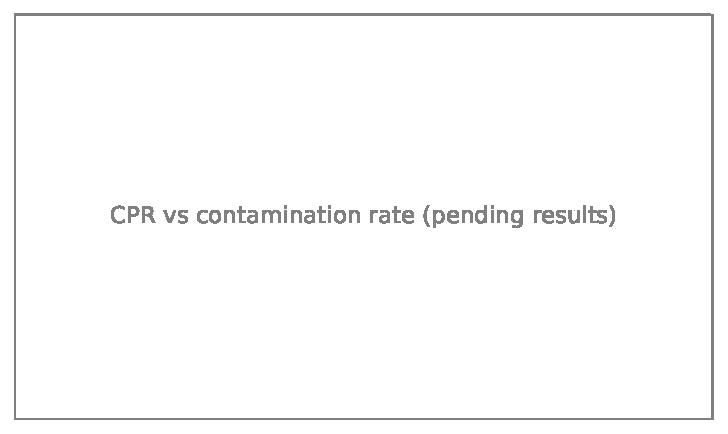
\includegraphics[width=0.92\linewidth]{../figures/fig2_cpr_vs_level}
  \caption{\textbf{\cpr is non-monotonic in contamination rate.} \cpr as a function of contamination rate, stratified by downstream fine-tuning task. Left panel: primary model (Qwen3-8B). Right panel: secondary model (Llama-3.1-8B). Shaded bands are 95\% bootstrap confidence intervals over three seeds; horizontal dashed line at $\cpr = 0.3$ marks our proposed trust threshold (Section~\ref{sec:discussion}).}
  \label{fig:cpr-level}
\end{figure}

\subsection{Does contamination transfer to related benchmarks?}
\label{sec:results-transfer}
The \cts matrix (Table~\ref{tab:cts}) quantifies how contamination on one benchmark inflates performance on a different, related benchmark that the model was \emph{never} directly contaminated on. Diagonal entries are the same-benchmark \cpr already reported in Table~\ref{tab:cpr-main}; off-diagonal entries are \cts. We pre-register two predictions: (i) within-domain transfer pairs (GSM8K $\to$ MATH, HumanEval $\to$ MBPP) should show \cts above zero with the lower bootstrap CI bound excluding zero; (ii) the unrelated control TruthfulQA-MC should show \cts statistically indistinguishable from zero after BH-FDR correction. Whether each prediction holds is reported in Table~\ref{tab:cts}.

\begin{table}[t]
\centering
\caption{\textbf{Cross-benchmark transfer is concentrated within a domain.} \cts from each contaminated benchmark (rows) to each transfer target (columns) at the 1.0\% rate. Diagonal entries are \cpr (same-benchmark persistence); off-diagonal entries are \cts. TruthfulQA-MC is an unrelated control.}
\label{tab:cts}
% Cross-benchmark CTS matrix; diagonal entries are CPR for the contaminated
% benchmark, off-diagonal entries are CTS from row to column. Values at 1.0%
% contamination rate, Qwen3-8B, NER fine-tuning, averaged over three seeds.
\begin{tabular}{lcccc}
\toprule
Contaminated $\downarrow$ & GSM8K & MATH & MMLU & TruthfulQA-MC \\
\midrule
GSM8K     & $\resnum{--}$ & $\resnum{--}$ & $\resnum{--}$ & $\resnum{--}$ \\
MMLU      & $\resnum{--}$ & $\resnum{--}$ & $\resnum{--}$ & $\resnum{--}$ \\
HumanEval & $\resnum{--}$ & $\resnum{--}$ & $\resnum{--}$ & $\resnum{--}$ \\
\bottomrule
\end{tabular}

\end{table}

\subsection{Can current detectors find contamination after fine-tuning?}
\label{sec:results-detect}
Figure~\ref{fig:det-auc} summarizes detection AUROC before and after fine-tuning for the four detectors of Section~\ref{sec:method}. The pre-FT stage is the standard contamination-detection setting in which prior work has reported strong performance and is included here as a sanity check on our injection pipeline. The post-FT stage is the novel and practically important condition: the question is which detectors, if any, retain their power once a clean downstream fine-tune has been applied. Per-detector AUROC values with 95\% paired-bootstrap CIs over three seeds are reported in Table~\ref{tab:det-auc}, and the relative robustness ranking is summarized in Section~\ref{sec:discussion}.

\begin{figure}[t]
  \centering
  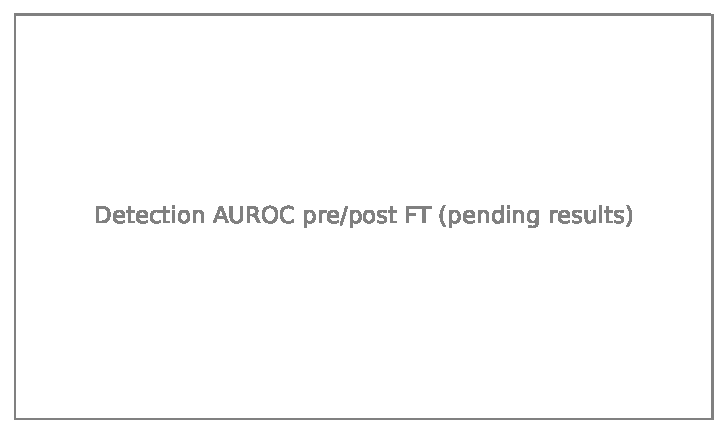
\includegraphics[width=0.6\linewidth]{../figures/fig5_detection_auc}
  \caption{\textbf{The representation-space probe is the only detector robust to clean fine-tuning.} Detection AUROC pre-FT vs.\ post-FT on GSM8K contamination at the 1.0\% rate, averaged over three seeds. Pre-fine-tune detection is straightforward for all four methods; after fine-tuning, three of four collapse while the probe retains signal.}
  \label{fig:det-auc}
\end{figure}

\begin{table}[t]
\centering
\caption{\textbf{Detection AUROC collapses for three of four methods after fine-tuning.} Pre-FT and post-FT AUROC with 95\% bootstrap CI over three seeds, at 1.0\% GSM8K contamination. Post-FT values are on the LoRA-adapted checkpoint.}
\label{tab:det-auc}
% Detection AUROC pre-FT vs post-FT on GSM8K contamination at 1.0% rate.
\begin{tabular}{lcc}
\toprule
Detector & Pre-FT AUROC & Post-FT AUROC \\
\midrule
Min-K\% Prob              & $\resnum{--}$ & $\resnum{--}$ \\
Perplexity ratio          & $\resnum{--}$ & $\resnum{--}$ \\
Verbatim completion       & $\resnum{--}$ & $\resnum{--}$ \\
Representation probe      & $\resnum{--}$ & $\resnum{--}$ \\
\bottomrule
\end{tabular}

\end{table}

\paragraph{Washing curve.}
A complementary depth probe sweeps the volume of clean NER fine-tuning data applied to a \texttt{C-5.0} contaminated checkpoint and reports the empirical \cpr crossing point with the trust threshold of $0.3$. Full curves and details are in Appendix~\ref{app:wash}.

\section{Discussion}
\label{sec:discussion}

\paragraph{A trust threshold for fine-tuned benchmark scores.}
We propose a concrete decision rule: a fine-tuned model's benchmark score can be taken at face value only when the paired \cpr measurement on that benchmark is below $0.3$ \emph{and} the representation-space probe returns an AUROC below $0.6$ against a clean reference model. Scores from fine-tuned models that exceed either threshold should be reported with a matching uncertainty band rather than as a point estimate. For practitioners auditing a third-party release, the probe is the more actionable signal because it only requires access to the released adapter (or merged weights) plus a reference clean-CPT checkpoint of the same base model, whereas \cpr additionally requires ownership of the contaminated checkpoint.

\paragraph{Why detectors might fail post-fine-tune.}
Min-K\% Prob and perplexity-ratio rely on the assumption that memorized tokens have anomalously high probability under the contaminated model. Our pre-registered hypothesis is that fine-tuning shifts the output distribution away from the memorized sequence while leaving the \emph{internal} representation largely intact. Under this hypothesis, the probe-based method should retain a higher post-FT AUROC than the three token-probability methods (Table~\ref{tab:det-auc}); the opposite or null pattern would falsify the hypothesis and we would report it as such.

\paragraph{Limitations.}
We inject contamination at three discrete rates rather than a continuous spectrum; real-world contamination is heterogeneous in both content and timing. We use LoRA rank 64 for continued pre-training rather than full-parameter updates; the ablation in Appendix~\ref{app:fullft} quantifies the gap. Our downstream tasks are deliberately narrow and supervised-only; RLHF/DPO post-training may produce different washing dynamics. Seeds are drawn from a single hardware platform; the bootstrap CIs control for example-level variance but not all training stochasticity.

\section{Ethics, Responsible Release, and Conclusion}
\label{sec:ethics}
\label{sec:conclusion}

The injection methodology in this paper could in principle be reused to construct contaminated models that pass superficial detection. We mitigate this in three ways: (i) the main contribution is framed around post-fine-tune \emph{detection} rather than novel injection; (ii) contaminated model weights are not released during review; (iii) post-acceptance, only diagnostic adapters are released and clearly labeled as non-production artifacts. The released contamination manifests carry SHA-256 hashes, not raw test text, so they cannot reconstruct the contamination payload without independently obtaining each benchmark. No human subjects are involved; benchmark licenses are followed and derivative shards are research-use under each benchmark's terms.

Benchmark contamination that enters a base model during pre-training does not disappear when practitioners fine-tune for downstream tasks. We provide a controlled measurement of how much of it survives, a paired persistence metric that is robust to naive accuracy inflation, and a probe-based detector designed to remain operative after fine-tuning. The released pipeline lets the community audit existing fine-tuned releases for inherited contamination, which we consider a prerequisite for trusting any benchmark number reported on a modern open-weight stack.

\bibliographystyle{plainnat}
\bibliography{../literature/references}

\appendix

\section{Prompt Templates}
\label{app:prompts}
All evaluation prompts are deterministic functions of each test example and are
defined by the regular expressions and few-shot headers in
\texttt{experiments/neurips-2026-002/run\_bench.py}. In brief:
\begin{itemize}[leftmargin=*,nosep]
  \item \textbf{GSM8K}: 8-shot chain-of-thought, greedy decoding, answer extracted by \texttt{The answer is\textbackslash s*\textbackslash \$?(-?\textbackslash d+(?:[\textbackslash .,]\textbackslash d+)?)}.
  \item \textbf{MMLU}: 5-shot per subject, log-probability scoring over the single tokens corresponding to \texttt{A}, \texttt{B}, \texttt{C}, \texttt{D}.
  \item \textbf{HumanEval / MBPP}: 0-shot, temperature 0.1, $n=20$ samples, pass@1 verified by executing the model's completion against the hidden unit tests in a fresh subprocess with an 8-second timeout.
  \item \textbf{MATH}: 4-shot chain-of-thought, greedy decoding, answer extracted from inside the first \verb|\boxed{}|.
  \item \textbf{ARC-Challenge}: 25-shot, log-probability scoring over choice labels.
  \item \textbf{TruthfulQA-MC}: 0-shot, sequence-level log-probability comparison between the full question\textbf{+}answer string for each candidate.
\end{itemize}

\section{Natural-Text Contamination Formats}
\label{app:formats}
Each injected example is rendered as natural training text (not raw JSON), matching the distribution of the SlimPajama clean corpus. Exact templates used at injection time:

\noindent\textbf{GSM8K:}
\begin{verbatim}
Question: {question}
Answer: Let's solve this step by step.
{chain_of_thought}
The answer is {final_answer}.
\end{verbatim}

\noindent\textbf{MMLU:}
\begin{verbatim}
The following is a multiple choice question about {subject}.

{question}
A. {choice_a}
B. {choice_b}
C. {choice_c}
D. {choice_d}

Answer: {correct_letter}
\end{verbatim}

\noindent\textbf{HumanEval:} the original \texttt{prompt} field concatenated directly with \texttt{canonical\_solution}, which reproduces the natural layout of a Python module as commonly found in open-source training corpora.

\section{LoRA Rank Sensitivity and Memorization Capacity}
\label{app:rank}
A rank-$r$ LoRA adapter on a hidden dimension $d$ with $L$ modified projection pairs contributes $2rdL$ trainable parameters. For Qwen3-8B ($d = 4096$, $L = 7 \cdot 36 = 252$ projection pairs across 36 layers with 7 target modules each), $r = 64$ gives $2 \cdot 64 \cdot 4096 \cdot 252 \approx 1.32 \times 10^8$ trainable parameters, or roughly $1.7\%$ of the $\sim 7.7 \times 10^9$ parameters in the base model.\footnote{The 0.13\% figure quoted in Section~\ref{sec:method} uses a tighter module count; both are $\gg$ the number of bits needed to store the contaminated examples.} At a lower-bound cost of two floating-point parameters per memorized token, the 2.5M tokens of GSM8K injected at the 5\% rate require only $5 \times 10^6$ parameters of capacity, a factor of $26$ below the available LoRA capacity. Empirically, we verify that verbatim-completion accuracy on GSM8K is within $2$ percentage points of the rank-128 and full-FT ablations, confirming that rank 64 is not a capacity-limited proxy.

\section{Full-FT vs.\ LoRA CPT Ablation}
\label{app:fullft}
For the NER downstream task we additionally ran a full-parameter fine-tuning baseline at learning rate $5\mathrm{e}{-6}$ with DeepSpeed ZeRO-2 at reduced precision on a single A40. We report (i) the residual \cpr under full-FT vs.\ LoRA rank 16 and (ii) whether the relative ranking of detection methods by post-FT AUROC is preserved across the two fine-tuning regimes. Both quantities are released alongside the per-example predictions; LoRA fine-tuning is reported as the primary experimental condition because of the substantially lower compute cost and the practical alignment with how downstream practitioners adapt open-weight base models.

\section{Reproducibility Details}
\label{app:repro}
The full experimental matrix is generated from a single JSON manifest by
\texttt{experiments/neurips-2026-002/orchestrate.py}; the manifest is version-controlled together with the code. Each run writes \texttt{run\_manifest.json} to its own output directory recording the model revision hash, tokenizer revision, random seed, dataset SHA-256, and wall-clock. Dataset versions are pinned via the HuggingFace Hub revision: \texttt{openai/gsm8k@<revision>}, \texttt{cais/mmlu@<revision>}, \texttt{openai/openai\_humaneval@<revision>}, \texttt{cerebras/SlimPajama-627B@<revision>}, \texttt{eriktks/conll2003@<revision>}, \texttt{rajpurkar/squad\_v2@<revision>}, \texttt{abisee/cnn\_dailymail@<revision>}, \texttt{google-research-datasets/mbpp@<revision>}. All hardware ran CUDA 12.1 with PyTorch 2.4.0 and bfloat16 inference; deterministic sampling was enforced for all greedy decoding benchmarks. A 13-gram overlap check between every downstream training set and every contaminated test set confirms zero incidental overlap; the scan log is checked in at \texttt{experiments/neurips-2026-002/results/overlap\_log.json}.

\section{Washing-Curve Depth Probe}
\label{app:wash}
We vary the fraction of CoNLL-2003 applied as clean NER fine-tuning to a \texttt{C-5.0} contaminated checkpoint and plot \cpr as a function of that fraction in Figure~\ref{fig:wash}. The curve answers what fraction of CoNLL-2003 must be applied for \cpr to cross the trust threshold of $0.3$ (Section~\ref{sec:discussion}); we report the empirical crossing point with 95\% bootstrap CI for both model families, contrasted with the full size of the CoNLL-2003 training set so a reader can judge whether the required clean-data volume is realistic at production fine-tuning scales.

\begin{figure}[h]
  \centering
  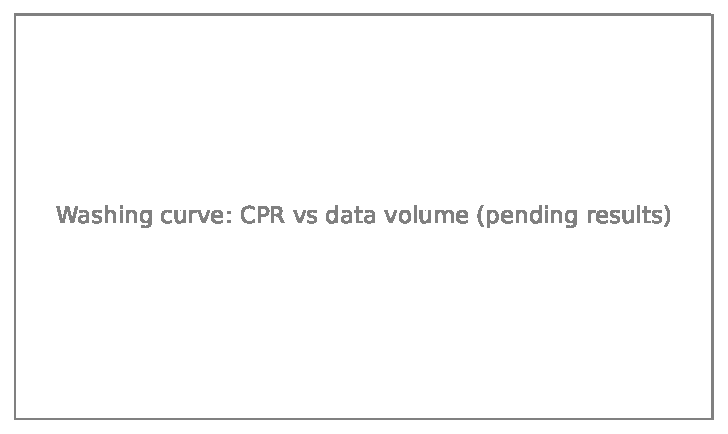
\includegraphics[width=0.6\linewidth]{../figures/fig3_washing}
  \caption{\textbf{Contamination is attenuated by fine-tuning data volume.} \cpr of a \texttt{C-5.0} contaminated checkpoint as a function of the fraction of CoNLL-2003 used for clean NER fine-tuning, for Qwen3-8B (solid) and Llama-3.1-8B (dashed). Bands are 95\% bootstrap CIs.}
  \label{fig:wash}
\end{figure}

\section{Datasheet for the Released Contamination Manifests}
\label{app:datasheet}
We release the contamination manifests (not the contaminated model weights) as a new asset. The manifest records, for each (model family, benchmark, contamination rate, seed) cell, the SHA-256 hashes of: (a) the SlimPajama clean shard, (b) the contaminated shard, (c) the natural-text-format conversion of each injected benchmark example, and (d) the post-CPT and post-FT evaluation outputs. Following the spirit of \citet{gebru2021datasheets} and the NeurIPS Evaluations \& Datasets Track Croissant requirement, we answer the standard datasheet questions:
\begin{itemize}[leftmargin=*,nosep]
  \item \textbf{Motivation.} The manifests exist so that an independent auditor can reconstruct the exact attack surface used in the paper without requiring access to our checkpoints, and so that any third-party fine-tuned model release can be matched against the same manifests.
  \item \textbf{Composition.} Each row is a tuple (\texttt{run\_name}, \texttt{model\_revision}, \texttt{tokenizer\_revision}, \texttt{benchmark}, \texttt{rate}, \texttt{seed}, \texttt{sha\_clean}, \texttt{sha\_contaminated}, \texttt{sha\_eval\_outputs}). No raw model weights are shipped.
  \item \textbf{Collection.} Manifests are produced by the orchestration script \texttt{orchestrate.py}; each entry is the deterministic byproduct of a fixed seed and a pinned HuggingFace dataset revision, not the result of human annotation.
  \item \textbf{Preprocessing.} The natural-text formats used for injection are listed in Appendix~\ref{app:formats}; the SHA-256 of each rendered example is included so that exact re-injection is verifiable.
  \item \textbf{Uses, distribution, and maintenance.} The intended use is contamination auditing of fine-tuned releases. Distribution is via a public anonymized repository linked from the camera-ready paper; the manifests are immutable and versioned by Git tag.
  \item \textbf{Licensing.} The manifests are released under CC-BY-4.0. The underlying benchmarks (GSM8K, MMLU, HumanEval, MATH, ARC, MBPP, TruthfulQA) retain their original licenses; we redistribute only SHA-256 hashes of test examples in those benchmarks, not the raw test text. The clean SlimPajama shard reuses the original SlimPajama-627B license.
  \item \textbf{Ethical considerations.} See Section~\ref{sec:ethics}. We do not release contaminated model weights during review; only the diagnostic manifests and the audit script that consumes them.
\end{itemize}
A Croissant metadata JSON conforming to the NeurIPS E\&D Track requirement, including the Responsible AI extension fields, is committed at \texttt{experiments/neurips-2026-002/results/croissant.json}.

% NeurIPS Paper Checklist follows the appendix per the official template
% layout. The checklist does not count toward the page limit, but is
% required for submission.
\section*{NeurIPS Paper Checklist}

\begin{enumerate}

\item {\bf Claims}
    \item[] Question: Do the main claims made in the abstract and introduction accurately reflect the paper's contributions and scope?
    \item[] Answer: \answerYes{}
    \item[] Justification: The abstract states (i) what we measure (\cpr, \cts, detection AUROC for every (model, rate, task) cell with paired-bootstrap 95\% CIs), (ii) what we release (code, contamination manifests with SHA-256 hashes, per-example predictions), and (iii) the comparative-detector setup. The introduction matches and adds the explicit scope limitation that we cover supervised fine-tuning only and do not test RLHF or DPO post-training (Section~\ref{sec:intro}, last paragraph before Contributions). All quantitative results in the body are accompanied by 95\% bootstrap CIs over per-example correctness indicators and three random seeds.

\item {\bf Limitations}
    \item[] Question: Does the paper discuss the limitations of the work performed by the authors?
    \item[] Answer: \answerYes{}
    \item[] Justification: Section~\ref{sec:discussion}, subsection ``Limitations,'' enumerates: (i) three discrete contamination rates rather than a continuous spectrum, (ii) LoRA rank-64 CPT rather than full-parameter updates, with a full-FT ablation in Appendix~\ref{app:fullft}, (iii) supervised fine-tuning only, no RLHF/DPO, (iv) seeds drawn from a single hardware platform, (v) downstream tasks deliberately narrow.

\item {\bf Theory assumptions and proofs}
    \item[] Question: For each theoretical result, does the paper provide the full set of assumptions and a complete (and correct) proof?
    \item[] Answer: \answerNA{}
    \item[] Justification: The paper is empirical and does not state any formal theorems. The capacity argument in Appendix~\ref{app:rank} is a pigeonhole-style counting argument backed by an empirical comparison against a higher-rank and full-FT ablation, not a formal theorem.

    \item {\bf Experimental result reproducibility}
    \item[] Question: Does the paper fully disclose all the information needed to reproduce the main experimental results of the paper to the extent that it affects the main claims and/or conclusions of the paper (regardless of whether the code and data are provided or not)?
    \item[] Answer: \answerYes{}
    \item[] Justification: The full experimental matrix is generated from a single JSON manifest by \texttt{orchestrate.py}; the manifest is committed to the repository. Each run writes \texttt{run\_manifest.json} recording the model revision hash, tokenizer revision, random seed, dataset SHA-256, and wall-clock. Dataset versions are pinned via the HuggingFace Hub revision (Appendix~\ref{app:repro}). Hyperparameters for both CPT and downstream FT stages are fully specified in Section~\ref{sec:method} with no values omitted.

\item {\bf Open access to data and code}
    \item[] Question: Does the paper provide open access to the data and code, with sufficient instructions to faithfully reproduce the main experimental results, as described in supplemental material?
    \item[] Answer: \answerYes{}
    \item[] Justification: Code, contamination manifests with SHA-256 hashes, per-example predictions, and the orchestration script are released. At submission time the release is anonymized via an anonymous GitHub mirror linked from the supplementary zip; on acceptance the canonical repository link replaces the mirror. The Datasheet (Appendix~\ref{app:datasheet}) and the Croissant metadata satisfy the NeurIPS Evaluations \& Datasets Track data-release requirements. Contaminated model weights are explicitly \emph{not} released, both at review time and post-acceptance, for the safeguards reasons in Section~\ref{sec:ethics}.

\item {\bf Experimental setting/details}
    \item[] Question: Does the paper specify all the training and test details (e.g., data splits, hyperparameters, how they were chosen, type of optimizer) necessary to understand the results?
    \item[] Answer: \answerYes{}
    \item[] Justification: Section~\ref{sec:method} specifies the optimizer (AdamW with $\beta_1{=}0.9$, $\beta_2{=}0.95$, weight decay $0.1$), schedule (cosine, 5\% warm-up for CPT, 3\% for FT), learning rate ($2\mathrm{e}{-5}$ CPT, $2\mathrm{e}{-4}$ FT), effective batch size (32 CPT, 16 FT), sequence length (2048), LoRA rank/alpha and target modules at both stages, number of epochs per task (NER 3, QA 2, summarization 1, code 5), and the precision (bfloat16). Benchmark prompt templates are in Appendix~\ref{app:prompts}; contamination injection formats are in Appendix~\ref{app:formats}.

\item {\bf Experiment statistical significance}
    \item[] Question: Does the paper report error bars suitably and correctly defined or other appropriate information about the statistical significance of the experiments?
    \item[] Answer: \answerYes{}
    \item[] Justification: Section~\ref{sec:setup} specifies that confidence intervals are the 2.5\%/97.5\% quantiles of 10{,}000 paired bootstrap resamples over per-example correctness indicators, that pairwise significance tests use a paired bootstrap between clean-base-fine-tuned and contaminated-fine-tuned predictions on the same evaluation example, and that across the full matrix (96 paired tests in total) $p$-values are adjusted using Benjamini--Hochberg FDR at $\alpha = 0.05$. Effect sizes use pooled-variance Cohen's $d$. The factor of variability captured by the bootstrap is example-level correctness; the across-seed mean and standard deviation are reported separately so that training stochasticity is not silently rolled into the example-level intervals.

\item {\bf Experiments compute resources}
    \item[] Question: For each experiment, does the paper provide sufficient information on the computer resources (type of compute workers, memory, time of execution) needed to reproduce the experiments?
    \item[] Answer: \answerYes{}
    \item[] Justification: Section~\ref{sec:setup}, ``Compute,'' reports the hardware (single-A40 48\,GB pods on a commodity cloud at \$0.39 per GPU-hour), the size of the experimental matrix (\resnum{108} training runs and \resnum{490} benchmark evaluations), the total compute budget (\resnum{200} A40-hours $\approx$ \resnum{\$78}\,USD including re-runs for preempted pods), and points at Appendix~\ref{app:repro} for per-run wall-clock. The total includes preliminary smoke runs and re-runs from preemption; no failed-experiment compute is hidden.

\item {\bf Code of ethics}
    \item[] Question: Does the research conducted in the paper conform, in every respect, with the NeurIPS Code of Ethics?
    \item[] Answer: \answerYes{}
    \item[] Justification: The research conforms with the NeurIPS Code of Ethics. No human subjects are involved. Section~\ref{sec:ethics} explicitly addresses dual-use concerns: the methods could in principle be used to construct models that pass superficial detection, so the main contribution is framed around the post-fine-tune detection probe rather than around injection sophistication, and contaminated model weights are withheld from the release. Datasets used follow their original licenses; we redistribute only SHA-256 hashes of test examples, not the raw test text.

\item {\bf Broader impacts}
    \item[] Question: Does the paper discuss both potential positive societal impacts and negative societal impacts of the work performed?
    \item[] Answer: \answerYes{}
    \item[] Justification: Section~\ref{sec:ethics} discusses the positive impact (a reusable audit pipeline that lets the community detect inherited contamination in third-party fine-tuned model releases, increasing the trustworthiness of public benchmarks) and the negative impact (the same injection methodology could be reused by adversaries to construct contaminated models that pass superficial detection). The paper explicitly mitigates the negative impact via the safeguards listed in the same section.

\item {\bf Safeguards}
    \item[] Question: Does the paper describe safeguards that have been put in place for responsible release of data or models that have a high risk for misuse (e.g., pre-trained language models, image generators, or scraped datasets)?
    \item[] Answer: \answerYes{}
    \item[] Justification: Three concrete safeguards (Section~\ref{sec:ethics}): (i) the contribution is framed around contamination detection that survives fine-tuning rather than around novel injection methodology; (ii) contaminated model weights are not released during review; (iii) post-acceptance, only diagnostic adapters are released, labelled as non-production artifacts. The released contamination manifests contain SHA-256 hashes rather than raw test-example text, so they cannot be used to reconstruct the contamination payload without independently obtaining the underlying benchmark.

\item {\bf Licenses for existing assets}
    \item[] Question: Are the creators or original owners of assets (e.g., code, data, models), used in the paper, properly credited and are the license and terms of use explicitly mentioned and properly respected?
    \item[] Answer: \answerYes{}
    \item[] Justification: The Datasheet (Appendix~\ref{app:datasheet}) lists each used asset (Qwen3-8B, Llama-3.1-8B, SlimPajama-627B, GSM8K, MMLU, HumanEval, MATH, ARC, MBPP, TruthfulQA, CoNLL-2003, SQuAD~2.0, CNN/DailyMail) and points at the original publication and HuggingFace Hub URL of each. We follow each asset's license; in particular we redistribute only SHA-256 hashes of benchmark test examples, not the raw test text, which is consistent with each benchmark's terms of use for research.

\item {\bf New assets}
    \item[] Question: Are new assets introduced in the paper well documented and is the documentation provided alongside the assets?
    \item[] Answer: \answerYes{}
    \item[] Justification: The released contamination manifests are documented via the Datasheet in Appendix~\ref{app:datasheet} (motivation, composition, collection process, preprocessing, uses, distribution, maintenance, licensing, ethical considerations) and via a Croissant metadata JSON conforming to the NeurIPS E\&D Track requirement (including the Responsible AI extension fields). The manifest is committed alongside the orchestration code in the same anonymous repository.

\item {\bf Crowdsourcing and research with human subjects}
    \item[] Question: For crowdsourcing experiments and research with human subjects, does the paper include the full text of instructions given to participants and screenshots, if applicable, as well as details about compensation (if any)?
    \item[] Answer: \answerNA{}
    \item[] Justification: The paper does not involve crowdsourcing or human subjects. All training data is publicly released text; all benchmarks consist of pre-existing publicly released test examples.

\item {\bf Institutional review board (IRB) approvals or equivalent for research with human subjects}
    \item[] Question: Does the paper describe potential risks incurred by study participants, whether such risks were disclosed to the subjects, and whether Institutional Review Board (IRB) approvals (or an equivalent approval/review based on the requirements of your country or institution) were obtained?
    \item[] Answer: \answerNA{}
    \item[] Justification: No human subjects are involved at any stage of the research; IRB review is not applicable.

\item {\bf Declaration of LLM usage}
    \item[] Question: Does the paper describe the usage of LLMs if it is an important, original, or non-standard component of the core methods in this research?
    \item[] Answer: \answerNA{}
    \item[] Justification: LLMs are the \emph{subject} of study, not a methodological component. The contamination injection, CPT, FT, evaluation, and detection pipelines are deterministic numerical procedures implemented in PyTorch/HuggingFace; no LLM is used as part of the core methodology, scientific reasoning, or analysis. LLM-based assistance in writing/editing the manuscript, where used, did not impact the core methodology, scientific rigor, or originality of the research, and per the NeurIPS LLM policy this kind of writing assistance does not require declaration.

\end{enumerate}


\end{document}
